


\section{STA Template correlation}

\begin{itemize}
    \item Idea for the two-pass test
    \item Template examples. Both ideal and template found with first-pass (STA height-only)
    \item Peformance for different N, \& comparison with previous method
\end{itemize}



\section{Fitting a full STA model}

\begin{itemize}
    \item Model design
    \item Iterative model fitting
    \item Problem of overfitting, and parameter-constraints to solve it
    \item An advantage: fit parameters (like transmission delay and time constants) are biologically ~meaningful
    \item Perfomance for different N, \& comparison with previous methods
\end{itemize}


\section{Linear regression of the upstroke}

All previous methods are STA-based, i.e. different windows are cut from the postsynaptic voltage signal -- one window for every presynaptic spike -- and these are averaged into one signal, which is then used for further analysis. The method described in this section does not use STAs. We still construct the spike-triggered windows, but we do not average them. Instead, we use them to construct a gigantic data matrix for use in a linear regression.

Every single timepoint on the x-axis (in relative time after the presynaptic spike) will correspond to multiple voltage values on the y-axis; namely one for every window. Whereas for an STA, every timepoint on the x-axis corresponds to just a single y-value (the average voltage).

Why a linear regression? As we saw with the STAs in previous sections, they do not look like a line. But their first part, the "upstroke", might be approximated by one.

Let's number our spike-triggered windows $1, 2, .., N$ (for a presynaptic spiketrain with $N$ spikes), and let's number the voltage values in window $i$ as $[y_{i,1}, y_{i,2}, .., y_{i,M}]$ (for a window length of $M$ samples long).\footnote{
    This window length $M$ is an important parameter. The window must be approximately as long as the upstroke of the STA/PSP: not longer (so that the shape is too complex to be fit by a line), nor shorter (so that there would not be enough data for a proper fit).
}
We will then perform the following linear regression:
\begin{align}
    \bm{y} \hspace{1.4em}
    &=  \hspace{1.6em}
    X  \hspace{2.2em}
    \bm{β}  \hspace{0.7em}
    + \hspace{1.4em}
    \bm{ε}
    \\[1em]
    \begin{bmatrix}
        y_{1,1} \\
        y_{1,2} \\
        \vdots \\
        y_{1,M} \\
        y_{2,1} \\
        y_{2,2} \\
        \vdots \\
        \vdots \\
        y_{N,M}
    \end{bmatrix}
    &=
    \begin{bmatrix}
        1 & 1 \\
        1 & 2 \\
        \vdots & \vdots \\
        1 & M \\
        1 & 1 \\
        1 & 2 \\
        \vdots & \vdots \\
        \vdots & \vdots \\
        1 & M
    \end{bmatrix}
    \begin{bmatrix}
        β_0 \\
        β_1
    \end{bmatrix}
    +
    \begin{bmatrix}
        ε_{1,1} \\
        ε_{1,2} \\
        \vdots \\
        ε_{1,M} \\
        ε_{2,1} \\
        ε_{2,2} \\
        \vdots \\
        \vdots \\
        ε_{N,M}
    \end{bmatrix}
\end{align}
I.e. we will regress voltage-after-spike against time-after-spike.

If we assume additive Gaussian noise, i.e.
\begin{equation} \label{eq:sampling_noise}
    ε_{i,j} \sim \mathcal{N}(0, σ^2)
\end{equation}
then the maximum-likelihood estimate $\hat{\bm{β}}$ of the regression parameters $\bm{β}$ is obtained through minimizing the mean squared error (MSE)\footnote{
    \url{https://statproofbook.github.io/P/slr-mle}
}
between our observed voltage values $\bm{y}$ and the fitted line $\hat{\bm{y}} = X \hat{\bm{β}}$:
\begin{equation}
    \hat{\bm{β}} = \argmin_{\bm{β}} || \bm{y} - X \bm{β} ||_2^2.
\end{equation}
Our linear regression problem has become standard ordinary least squares (OLS) regression, for which a closed-form solution exists (the so-called normal equations: $\hat{\bm{β}} = (X^T X)^{-1} X^T \bm{y}$).
As is standard practice and for numerical stability ("don't explicitly invert a matrix if not needed"), we instead find the optimal intercept ($\hat{β}_0$) and slope ($\hat{β}_1$) of our linear fit through an implicit solution using QR-factorization, via Julia's left-division operator: \texttt{$\hat{\bm{β}}$ = X \textbackslash \ y}.

From this linear fit we thus obtain a slope $\hat{β}_1$. To use our regression as a connection test, we will perform a hypothesis test on this slope. The null hypothesis is that this slope is zero ($H_0: \hat{β} = 0$): the voltage of the tested neuron does not react to spikes of the other tested neuron, and on average it stays flat.

If the slope $β_1$ really were $0$, then we would expect the fitted slope $\hat{β}_1$ to be distributed normally around $0$, as follows:\footnote{
    \url{https://gregorygundersen.com/blog/2021/09/09/ols-hypothesis-testing/}
}
\begin{equation} \label{eq:slope_distrib}
    \hat{β}_1 \sim \mathcal{N}(0, σ^2 [Q]_{2,2})
\end{equation}
where $σ^2$ is the variance of the sampling noise (\cref{eq:sampling_noise}), and $[Q]_{2,2}$ is the second diagonal element of the 'cofactor matrix' $Q$,\footnote{
    The indices are off by one ($\hat{β}_1$ vs $[Q]_{2,2}$), because the intercept in linear regression is conventionally called $β_0$, and so we start numbering the elements of $\bm{β}$ from $0$; but we number the elements of other vectors/matrices from $1$.
}
which is the inverse of the Gram matrix $X^T X$:
\begin{equation}
    Q = (X^T X)^{-1}
\end{equation}

We do not know what the sampling noise $σ^2$ is, but we have a maximum-likelihood estimate $\hat{σ}^2$ for it,\footnote{\url{https://statproofbook.github.io/P/slr-mle}} namely the MSE of the fit:
\begin{equation}\label{eq:σhat}
    \hat{σ}^2 = || \bm{y} - X \bm{\hat{β}} ||_2^2
\end{equation}

Our final test statistic $t$ to determine whether there is a connection from neuron A
to neuron B is then the slope of the fit (of B's voltage after neuron A's spikes), normalized by how noisy the parameter fit is:
\begin{equation}
    t = \hat{β}_1 / \hat{σ}_{\hat{β}_1}
\end{equation}
where $\hat{σ}_{\hat{β}_1}$ is the standard error of the slope (\cref{eq:slope_distrib} with \cref{eq:σhat}):
\begin{equation}
    \hat{σ}_{\hat{β}_1} = \sqrt{\hat{σ}^2 [Q]_{2,2}}
\end{equation}

Unlike in \cref{eq:slope_distrib}, $t$ is no longer strictly normally distributed.\footnote{
    Instead, it follows a Student's $t$-distribution, with $n - p$ degrees of freedom, where $n = M · N$ is the number of datapoints, and $p = 2$ is the number of parameters of the regression ($β_0$ and $β_1$).
}
But when the number of datapoints is quite large, as is the case here, the $t$-distribution becomes practically normal, and our test statistic $t$ will follow the standard normal distribution under the null hypothesis ("the slope is zero").

We can (and do) use this $t$-value as-is in our connection test, for the threshold sweep.\\
Additionally, if our assumptions (linear data-generating process, additive Gaussian noise) would be correct,\footnote{They are not.}
we could also assign an actual probability (a $p$-value) to observing slopes as extreme as observed. Because $t$ follows the standard normal distribution under the null-hypothesis, and with $\phi(x)$ the cumulative probability function of this distribution, we have: $p = 2\ \phi(-|t|)$: the probability that a sample smaller than $-|t|$ or larger than $|t|$ is drawn.

% \footnote{
%     Besides the maximum-likelihood estimator $\hat{σ}^2$, there is also a Bessel-corrected estimator of $σ^2$, namely $s^2 = \frac{n}{n-p} \hat{σ}^2$ (with $p = 2$ the number of parameters in the regression). Unlike $\hat{σ}^2$, this is an unbiased estimator ($\mathbb{E}[s^2] = σ^2$); "but it has a higher MSE".
% }

% \begin{itemize}
%     \item Non-STA method: concatenated individual windows as (X, y)
%     \item Examples of pooled windows, and fits
%     \item Mention the problem of unknown transmission delays
%     \item Perfomance for different N, \& comparison with previous methods
% \end{itemize}

\Cref{fig:N_sweep__AUC__upstroke_vs_STA} shows the performance of the described linear regression method, for different number of inputs $N$, and compared to the STA height method.

\begin{figure}
    \subfloat{
        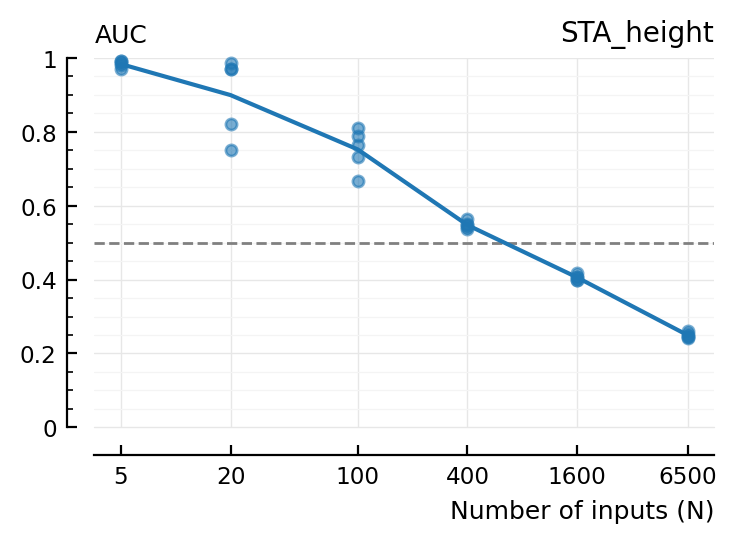
\includegraphics[w=0.72]{N_sweep__AUC__STA_height}
        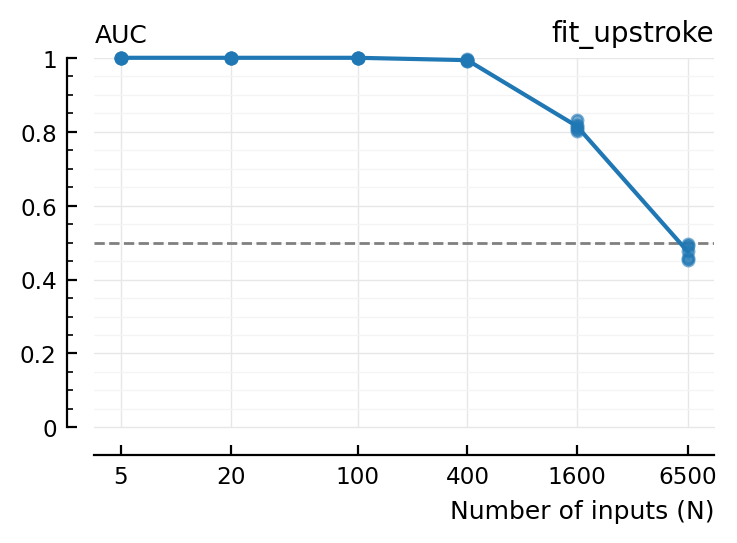
\includegraphics[w=0.72]{N_sweep__AUC__upstroke}
    }
    \captionn
        {Line fit outperforms STA height as connection test}
        {AdEx neuron, 10-minute recording, no voltage imaging noise,  5 different seeds (blue dots). All inputs are tested, instead of just the highest firing ones, in addition to 100 random unconnected spiketrains. AUC chance level is at $0.252$ (as in \cref{fig:AUC_chance_level}). \\
        Source: \nburl{2023-04-11__Nto1_AdEx_conntest_methods_comparison}.}
    \label{fig:N_sweep__AUC__upstroke_vs_STA}
\end{figure}



% \section{Clustering, \& Hierarchical model fitting}

% \begin{itemize}
%     \item (Time-permitting)
% \end{itemize}


% \section{Zhou/Cai's `Spike-triggered regression'}

% \begin{itemize}
%     \item (Time-permitting)
% \end{itemize}


\FloatBarrier
\section{Computational cost}

\begin{itemize}
    \item Timings of each method, extrapolation for larger number of tested connections
\end{itemize}

\section{Summary}

\begin{itemize}
    \item Conclusions of the N-to-1 experiment
    \item Leadup to the network experiments: what we could not yet test (the problem of indirect connections, as e.g. identified in the connectomics challenge)
\end{itemize}
